\documentclass[fr]{../../../eplsummary}

\usepackage{../../../eplmath}
\usepackage{multirow}
\usepackage{float}
\usepackage{tikz}
\usepackage{tabularx}
\usepackage[french, ruled, vlined]{algorithm2e}

\usetikzlibrary{matrix}

\SetKwComment{Comment}{$\triangleright$\ }{}
\SetKw{KwDownTo}{down to}

\graphicspath{{img/}}

\newcommand{\Cmn}{\C^{m \times n}}
\newcommand{\Cmm}{\C^{m \times m}}
\newcommand{\Rmn}{\R^{m \times n}}
\newcommand{\Rmm}{\R^{m \times m}}
\newcommand{\Cn}{\C^{n}}
\newcommand{\Cm}{\C^{m}}
\newcommand{\Rm}{\R^{m}}
\newcommand{\frob}[1]{\norm{#1}_{\textnormal{F}}}

\DeclareMathOperator{\nullspace}{null}
\DeclareMathOperator{\Image}{Im}
\DeclareMathOperator{\range}{range}
\DeclareMathOperator{\rank}{rank}
\DeclarePairedDelimiterX{\inp}[2]{\langle}{\rangle}{#1, #2}
\DeclareMathOperator{\tr}{tr}
\DeclareMathOperator{\sign}{sign}

\hypertitle[']{Analyse numérique}{5}{INMA}{1170}
{Gilles Peiffer}
{François Henrotte et Jean-François Remacle}

% TODO annexe Gmsh (CM2)?
% TODO check for reorganisation?
% TODO explain the last part of CM3 better, cf. slides

\section{Fondements}
Dans ce chapitre, nous allons étudier
les bases de l'algèbre linéaire\footnote{\textit{Pun intended\dots}}.
L'algèbre linéaire est l'étude de l'équation
\[
Ax = b\,.
\]
Il y a quatre façons de voir cette équation:
\begin{enumerate}
	\item Comme un \emph{produit matrice-vecteur}, où
	\[
	A \in \Cmn\,, \quad x \in \Cn\,, \quad b \in \Cn\,.
	\]
	\item Comme une \emph{expression tensorielle}:
	\[
	b_i = \sum_{j=1}^{n} a_{ij}x_i\,,
	\]
	où $a_{ij}$ est l'entrée
	à la $i$\ieme{} ligne
	et la $j$\ieme{} colonne de $A$.
	\item Comme disant que
	\emph{$b$ est dans le \textbf{column space} de $A$}\footnote{Espace vectoriel sous-tendu par les colonnes de $A$.},
	et est donc une combinaison linéaire des colonnes de $A$.
	\[
	b = Ax = \sum_{j=1}^{n} x_j a_j\,,
	\]
	où $a_j$ est la $j$\ieme{} colonne de $A$.
	\item Comme une \emph{application linéaire} de $\Cn$ dans $\Cm$:
	\begin{align*}
	A \colon \Cn &\to \Cm\,,\\
	x &\mapsto Ax\,.
	\end{align*}
	On a donc les propriétés suivantes:
	\[
	\begin{array}{rcl@{\quad}l}
		A(x+y) & = & A(x) + A(y)\,, & \quad \forall x,y \in \Cn\,,\\
		A(\alpha x) & = & \alpha A(x)\,, & \quad \forall x \in \Cn\,,
		\quad \alpha \in \C\,.
	\end{array}
	\]
\end{enumerate}

\subsection{Produit matrice-matrice}
Le produit matrice-matrice
\[
B = AC\,, \quad B \in \C^{\ell \times n}\,,\quad A \in \C^{\ell \times m}\,,\quad C \in \Cmn
\]
est une généralisation du produit matrice-vecteur vu précédemment.
On peut également l'écrire
\begin{align*}
	b_{ij} &= \sum_{k=1}^{m} a_{ik}c_{kj}\,.
\end{align*}
Chaque colonne de $B$ est une combinaison linéaire
des colonnes de $A$.

\subsection{Définitions}
\begin{mydef}[Column space]
	Le \emph{column space} d'une matrice $A \in \Cmn$,
	également noté $\range(A)$ est défini comme
	\[
	\range(A) = \mathrm{span}\{a_1, a_2, a_3, \dots, a_n\}\,.
	\]
\end{mydef}
\bigbreak
\begin{mydef}[Kernel]
	Le \emph{kernel} (\emph{noyau}, encore appelé \emph{null space}) d'une matrice $A \in \Cmn$
	est défini comme
	\[
	\nullspace(A) = \set{x \in \Cn \suchthat Ax = 0}\,.
	\]
	Les composantes de chaque vecteur de $\nullspace(A)$
	sont les coefficients d'une combinaison linéaire nulle
	des colonnes de $A$.
	\[
	Ax = 0 \iff \sum_{j=1}^{n} x_j a_j = 0\,.
	\]
\end{mydef}
\bigbreak
\begin{mydef}[Rang]
	Le \emph{rang} d'une matrice $A \in \Cmn$
	est défini comme la dimension de $\range(A)$:
	\[
	\rank(A) = \dim(\range(A))\,.
	\]
	Les espaces vectoriels sous-tendus
	par les lignes et les colonnes d'une matrice (carrée ou rectangulaire)
	ont toujours la même dimension.
	On appelle rang de la matrice $A$ cette dimension.
	On a donc nécessairement
	\[
	\rank(A) \le \min(m,n)\,.
	\]

	On dit qu'une matrice est \emph{de plein rang} lorsque
	\[
	\rank(A) = \min(m,n)\,.
	\]
	Une matrice est de plein rang si et seulement si
	jamais deux vecteurs différents de son domaine n'ont la même image.
	Cela implique que l'application
	\[
	A \colon \Cn \to \range(A) \subseteq \Cm
	\]
	est bijective\footnote{La démonstration est en page 7 du livre.}.
	% TODO add bib reference, maybe put this in an appendix?

	Il n'y a qu'une seule matrice \emph{de rang zéro} par dimension:
	la matrice nulle.

	Pour ce qui en est des matrices \emph{de rang un},
	prenons les vecteurs suivants:
	\begin{align*}
		u &\in \C^{m \times 1}\,,\\
		v &\in \C^{1 \times n}\,.
	\end{align*}
	Leur produit s'écrit
	\[
	\big(uv\big)_{ij} = u_i v_j\,.
	\]
	Cette matrice $\big(uv\big)_{ij}$ est de rang un,
	car toutes ses colonnes sont multiples de $u$.
\end{mydef}
\bigbreak
\begin{mydef}[Matrice inversible]
	Une matrice carrée $A \in \Cmm$ est \emph{inversible}
	si elle satisfait les propositions ci-dessous.
	Toutes les propositions suivantes sont équivalentes:
	\begin{enumerate}[label=(\alph*)]
		\item $A$ est inversible;
		\item $\rank(A) = m$ ($A$ est de plein rang);
		\item $\range(A) = \Cm$;
		\item $\nullspace(A) = \{0\}$ (et \emph{non pas} $\emptyset$);
		\item $0$ n'est pas une valeur propre de $A$;
		\item $0$ n'est pas une valeur singulière de $A$;
		\item $\det(A) \ne 0$.
	\end{enumerate}
\end{mydef}
\bigbreak
\begin{mydef}[Matrice adjointe]
	Si $A \in \Cmn$, la \emph{matrice adjointe} de $A$,
	notée\footnote{Une autre notation possible est $A^{\dag}$.} $A^*$,
	est la matrice obtenue:
	\begin{itemize}
		\item en prenant le complexe conjugué de chaque coefficient;
		\item en permutant lignes et colonnes.
	\end{itemize}
	Remarquons que si $A$ est réelle, $A^* = A^T$.
\end{mydef}
\subsection{Produit scalaire}
Un \emph{produit scalaire} (ou \emph{produit intérieur})
est une opération bilinéaire
\[
\inp{\cdot}{\cdot} \colon \Cm \times \Cm \to \C
\]
telle que
\[
x^* y = \sum_{i=1}^{m} \widebar{x}_i y_i\,,
\]
où $\widebar{x}_i$ est l'entrée $i$ du complexe conjugué de $x$.

Reprenons nos vecteurs $u \in \C^{1 \times m}$
et $v \in \C^{m \times 1}$.
On a que
\[
uv = \sum_{i=1}^{m} u_i v_i\,.
\]
Comme l'opération est bilinéaire,
on a
\[
\renewcommand{\arraystretch}{1.5}
\begin{array}{rcl@{\quad}l}
	\big(x_1 + x_2\big)^* y & = & x_1^* y + x_2^* y\,, & \forall x_1, x_2, y \in \Cm\,,\\
	x^* \big(y_1 + y_2\big) & = & x^* y_1 + x^* y_2\,, & \forall x, y_1, y_2 \in \Cm\,,\\
	\big(ax\big)^* by & = & \widebar{a}b x^* y\,, & \forall a,b \in \C\,, \quad \forall x,y \in \Cm\,.
\end{array}
\]
\subsubsection{Longueur d'un vecteur}
Avec ce produit scalaire,
il est possible de définir la longueur d'un vecteur:
\[
\norm{x} = \sqrt{x^* x}\,, \quad \textnormal{si } x\in \R^{m}\,.
\]

\subsubsection{Angle entre deux vecteurs}
Le produit scalaire permet aussi
de définir l'angle entre deux vecteurs:
\[
\cos \alpha = \frac{x^* y}{\norm{x}\norm{y}}\,.
\]
\subsubsection{Orthogonalité}
Grâce au produit scalaire,
on peut définir le concept d'orthogonalité
\begin{itemize}
	\item de deux vecteurs:
	\[
	x^* y = 0 \iff y^* x = 0\,,
	\]
	\item d'un ensemble $\mathcal{S}$ de vecteurs:
	\[
	x^* y = 0\,, \quad \forall x,y \in \mathcal{S} \suchthat x \ne y \implies \textnormal{ils sont linéairement indépendants,}
	\]
	\item de deux ensembles $\mathcal{S}$ et $\mathcal{S}'$
	de vecteurs non nuls:
	\[
	x^* y = 0\,,\quad \forall x \in \mathcal{S}\,,\quad \forall y \in \mathcal{S}'\,.
	\]
\end{itemize}
\subsubsection{Décomposition orthogonale}
Soit un ensemble $\mathcal{Q} = \{q_1,q_2,\dots,q_n\}$ de vecteurs orthonormés
formant une base orthonormée
pour un sous-espace de dimension $n \le m$ de $\Cm$.
On a alors\footnote{Où $\delta_{ij}$ est le \emph{symbole de Kronecker}.}
\[
q_i^* q_j = \delta_{ij}\,,\quad i,j = 1,\dots,n\,.
\]
Soit $v \in \Cm$.
On a la décomposition orthogonale
\begin{align*}
v &= r + \sum_{i=1}^{n} q_i^* v q_i\\
&= r + \sum_{i=1}^{n} q_i q_i^* v\,,
\end{align*}
avec $q_i^* r = 0$,
c'est-à-dire $r \perp \mathcal{Q}$.
\subsubsection{Matrice unitaire}
Une matrice unitaire est une matrice carrée vérifiant
\[
Q^* = Q^{-1} \iff Q^* Q = I\,,
\]
qui s'écrit également
\[
q_1^* q_2 = \delta_{ij}\,,
\]
en termes des colonnes de $Q$.
Les colonnes d'une matrice unitaire de $\Cmm$
forment une base orthonormée pour $\Cm$.
\subsubsection{Isométrie}
Une matrice unitaire laisse le produit scalaire invariant:
\[
\big(Qx\big)^* Qy = x^* y\,.
\]
Les longueurs des vecteurs et les angles qu'ils forment
sont donc également invariants\footnote{En mécanique des solides déformables,
cela donne lieu aux rotations et aux réflexions
selon que $\det(Q)$ soit $1$ ou $-1$ respectivement.}.
\subsection{Norme vectorielle}
Une norme vectorielle est une fonction
\[
\norm{\cdot} \colon \Cn \to \R
\]
satisfaisant les trois hypothèses suivantes:
\begin{itemize}
	\item \emph{séparation}: $\norm{x} \ge 0$
	avec l'égalité si et seulement si $x = 0$;
	\item \emph{inégalité triangulaire}: $\norm{x+y} \le \norm{x} + \norm{y}$;
	\item \emph{homogénéité absolue}: $\norm{ax} = \abs{a}\norm{x}\,,\quad \forall a \in \C$.
\end{itemize}

\begin{myrem}
	\emph{Le produit scalaire n'est donc pas une norme},
	car il ne satisfait pas la deuxième hypothèse.
	Cependant, sa racine carrée l'est.
\end{myrem}

Il existe beaucoup de normes différentes,
comme par exemple les $p$-normes (ou $\ell^p$-normes):
\begin{itemize}
	\item la norme $\ell^1$ définie par
	\[
	\norm{x}_1 \coloneqq \sum_i \abs{x_i}\,;
	\]
	\item la norme $\ell^2$ définie par
	\[
	\norm{x}_2 \coloneqq \sqrt{\sum_i x_i^2}\,;
	\]
	\item la norme $\ell^p$ définie par
	\[
	\norm{x}_p \coloneqq \left(\sum_i \abs{x_i}^p\right)^{1/p}\,;
	\]
	\item la norme $\ell^{\infty}$ définie par
	\[
	\norm{x}_\infty \coloneqq \max_i \abs{x_i}\,.
	\]
\end{itemize}
On peut donner une représentation graphique de ces normes vectorielles.
On définit pour cela les \emph{boules unitaires} (\emph{unit balls}):
\[
B_p^m = \set[\big]{x \in \Cm \suchthat \norm{x}_p \le 1}\,.
\]
\begin{figure}[H]
	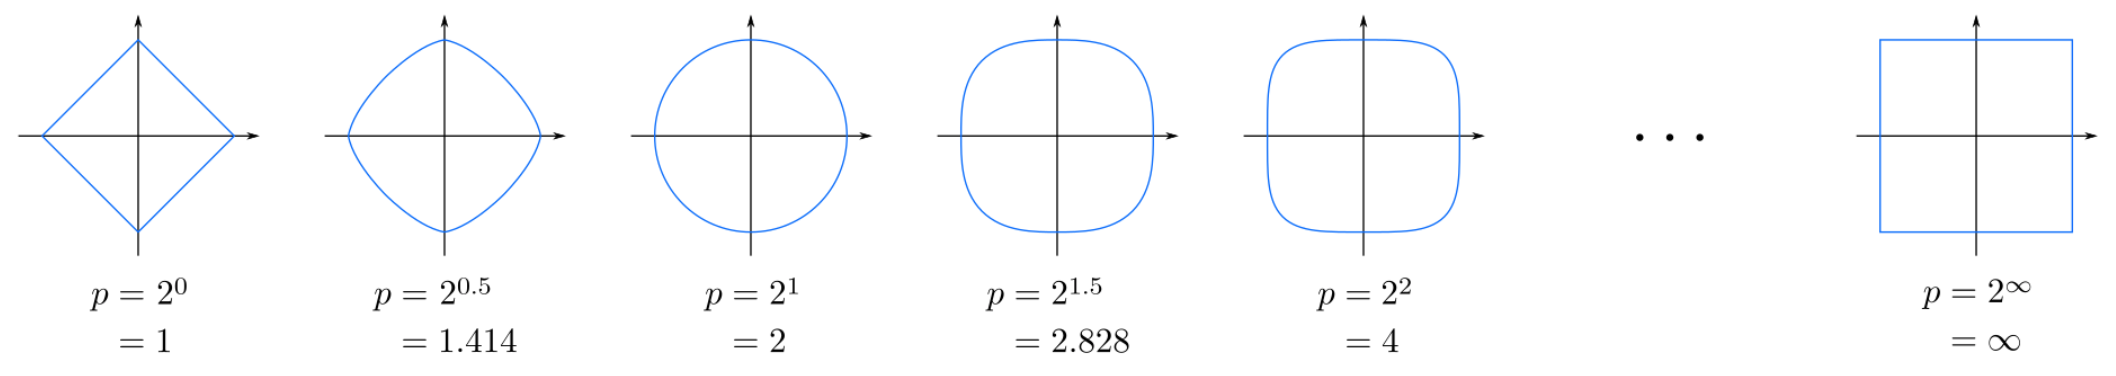
\includegraphics[width=\textwidth]{unit_balls.png}
	\caption{Une visualisation des boules $B_p^1$ pour $p \in \intervalco{1}{+\infty}$.}
	\label{fig:unit_balls}
	% TODO bib ref (wikipedia; unit ball)
\end{figure}
Comme on le voit sur la figure,
\[
B_p^m \subsetneq B_q^m\,,\quad \forall p < q\,.
\]
\subsection{Norme matricielle}
La norme matricielle induite par une norme vectorielle
est une norme pour les matrices
regardées comme des opérateurs sur les vecteurs.
Soit $A \in \Cmn$ un opérateur $A \colon \Cn \to \Cm$
et $\norm{\cdot}_{(m)}$ et $\norm{\cdot}_{(n)}$ deux normes vectorielles
respectivement sur $\Cm$ et $\Cn$.
On définit la norme matricielle $\norm{\cdot}_{(m,n)}$
induite par ces normes vectorielles par
\[
\norm{A}_{(m,n)} \coloneqq \sup_{x \in \Cn \setminus \{0\}} \frac{\norm{Ax}_{(m)}}{\norm{x}_{(n)}}\,.
\]
Comme toute norme doit satisfaire l'hypothèse d'homogénéité absolue,
et que $A$ est linéaire,
on voit que la norme de $x$ n'intervient pas dans la norme matricielle.
On peut également définir cette norme sans division:
\[
\norm{A}_{(m,n)} \coloneqq \sup_{x \in B_p^m} \norm{Ax}_{(m)}\,.
\]
On a l'égalité pratique suivante:
\[
\norm{A}_{(m, n)} \ge \frac{\norm{Ax}_{(m)}}{\norm{x}_{n}}\,.
\]

\subsubsection{$\norm{A}_1$}
\label{sec:1-norm}
% TODO cite example 3.3 in book
Soit la 1-norme matricielle $\norm{\cdot}_1$
induite par les normes vectorielles
$\norm{\cdot}_{(m)} = 1$ et $\norm{\cdot}_{(n)} = 1$.
Soit $A \in \Cmn$.
On prend $x \in B_{1}^{n}$,
et on écrit (où $a_j$ est la $j$\ieme{} colonne de $A$)
\begin{align*}
\norm{Ax}_1 &= \norm{\sum_{j=1}^{n} x_j a_j}_1 \\
&\le \sum_{j=1}^{n} \abs{x_j} \norm{a_j}_1 \\
&\le \max_{1 \le j \le n} \norm{a_j}_1\,.
\end{align*}
On en déduit que
\[
\norm{A}_1 \le \max_{1 \le j \le n} \norm{a_j}_1\,.
\]
Si on choisit $x = e_j$,
où $j$ maximise $\norm{a_j}_1$,
on atteint cette borne,
et donc la norme matricielle est le ``\emph{maximum column sum}'':
\[
\norm{A}_1 = \max_{1 \le j \le n} \norm{a_j}_1\,.
\]

\subsubsection{$\norm{A}_{\infty}$}
% TODO cite example 3.4 in book
Soit $A \in \Cmn$.
On prend $x \in B_{\infty}^{n} \implies \abs{x_j} \le 1 \quad \forall j$.
\begin{align*}
	\norm{Ax}_{\infty} &= \norm{\sum_{j=1}^{n} x_j a_j}_{\infty} \\
	&= \sum_{j=1}^{n} \norm{x_j a_j}_{\infty} \\
	&\le \sum_{j=1}^{n} \abs{x_j} \norm{a_j}_{\infty} \\
	&= \sum_{j=1}^{n} \abs{x_j} \max_{1 \le i \le m} a_{ij} \\
	&\le \sum_{j=1}^{n} \max_{1 \le i \le m} a_{ij} \\
	&= \max_{1 \le i \le m} \sum_{j=1}^{n} \abs{a_{j}} \\
	&= \max_{1 \le i \le m} \norm{a_i^*}_1\,.
\end{align*}
On applique le même raisonnement qu'à la \sectionref{1-norm}
pour trouver que la borne est serrée et égale au ``\emph{maximum row sum}'':
\[
\norm{A}_{\infty} = \max_{1 \le i \le m} \norm{a_i^*}_1\,.
\]

\subsubsection{Borner $\norm{AB}$}
Soient $\norm{\cdot}_{(\ell)}$,
$\norm{\cdot}_{(m)}$ et $\norm{\cdot}_{(n)}$
des $p$-normes vectorielles pour $\C^{\ell}$, $\Cm$ et $\Cn$ respectivement.
Soient $A \in \C^{\ell \times m}$ et $B \in \Cmn$.
On sait que
\begin{align*}
\norm{ABx}_{(\ell)} &\le \norm{A}_{(\ell, m)} \norm{Bx}_{(m)}\\
&\le \norm{A}_{(\ell, m)} \norm{B}_{(m, n)} \norm{x}_{(n)}\,.
\end{align*}
On trouve alors
\[
\norm{AB}_{(\ell, n)} \le \norm{A}_{(\ell, m)} \norm{B}_{(m, n)}\,.
\]
Notons qu'en général, cette inégalité n'est pas serrée.

\subsection{Inégalités de Cauchy-Schwarz et de Hölder}
Calculer les $p$-normes matricielles avec $p \ne 1, \infty$ est compliqué,
et afin de résoudre ce problème,
on note que les produits intérieurs peuvent être bornés
en utilisant des $p$-normes.
Soient $p$ et $q$ tels que
\[
\frac{1}{p} + \frac{1}{q} = 1\,, \quad 1 \le p, q \le \infty\,.
\]
L'\emph{inégalité de Hölder} dit alors que,
pour tout vecteurs $x$ et $y$,
\[
\abs{x^* y} \le \norm{x}_p \norm{y}_q\,.
\]
Dans le cas particulier $p = q = 2$,
on a l'\emph{inégalité de Cauchy-Schwarz}:
\[
\abs{x^* y} \le \norm{x}_2 \norm{y}_2\,.
\]
Ces deux bornes sont serrées.

\begin{myrem}
	Deux remarques sont à faire ici:
	\begin{itemize}
		\item Il ne faut pas confondre cette inégalité
		avec l'inégalité triangulaire qui implique une somme.
		\item Cette inégalité n'est valable que pour certaines normes.
	\end{itemize}
\end{myrem}

\subsection{Norme de Frobenius}
La norme de Frobenius\footnote{Également appelée norme de Hilbert-Schmidt.} d'une matrice
n'est pas induite par une norme vectorielle.
Pour être une norme matricielle,
il suffit que la norme vérifie les trois propriétés des normes vectorielles,
appliquées dans l'espace vectoriel des matrices, de dimension $mn$.
La norme de Frobenius est définie comme
\begin{align*}
\frob{A} &= \left(\sum_{i=1}^{m} \sum_{j=1}^{n} \abs{a_{ij}^2}\right)^{1/2} \\
&= \left(\sum_{j=1}^{n} \norm{a_{j}}_2 \right)^{1/2} \\
&= \sqrt{\tr(A^* A)}\,.
\end{align*}

\begin{mytheo}[Invariance sous multiplication unitaire]
La norme de Frobenius et la $2$-norme matricielle sont invariantes
sous multiplication par une matrice unitaire,
c'est-à-dire que pour tout $A \in \Cmn$, et $Q \in \Cmm$ unitaire,
on a
\[
\norm{QA}_2 = \norm{A}_2 \quad \textnormal{et} \quad \frob{QA} = \frob{A}\,.
\]
\end{mytheo}

La norme de Frobenius peut être utilisée pour borner un produit de matrices.
Posons $C = AB$ avec $C \in \C^{n \times m}$
dont les entrées sont les $c_{ik} = a_i^* b_j$.
Par l'inégalité de Cauchy-Schwarz,
on a alors $\abs{c_{ij}} \le \norm{a_i}_2 \norm{b_j}_2$.
En mettant au carré des deux cotés et en sommant, on trouve
\begin{align*}
	\frob{C}^2 = \frob{AB}^2 &= \sum_{i=1}^{n} \sum_{j=1}^{m} \abs{c_{ij}^2} \\
	&\le \sum_{i=1}^{n} \sum_{j=1}^{m} \left(\norm{a_i}_2 \norm{b_j}_2 \right)^2 \\
	&= \sum_{i=1}^{n} \left( \norm{a_i}_2 \right)^2 \sum_{j=1}^{m} \left( \norm{b_j}_2 \right)^2 \\
	&= \frob{A}^2 \frob{B}^2\,.
\end{align*}

\section{Factorisation QR}
\subsection{Projecteurs}
\begin{mydef}[Projecteur]
	Un \emph{projecteur} est une matrice carrée $P$
	qui satisfait l'équation
	\[
	P^2 = P\,.
	\]
	Une telle matrice est également appelée \emph{idempotente}.
	On distingue les projecteurs orthogonaux et non orthogonaux.
	Un projecteur n'a que deux valeurs propres potentielles: $0$ et $1$.
	Si le projecteur $P$ est symétrique, alors
	\[
	\Image P \perp \ker P\,.
	\]
\end{mydef}

On définit un projecteur ``fondamental''\footnote{Nom donné par le professeur.}
tel que
\begin{align*}
P &= \frac{vv^*}{\norm{v}_2^2} = \frac{vv^*}{v^* v} \\
\implies P^2 &= \frac{(v v^*) (v v^*)}{\norm{v}_2^4} = \frac{v v^* \norm{v}_2^2}{\norm{v}_2^4} = \frac{vv^*}{\norm{v}_2^2} = P\,.
\end{align*}

On définit également un projecteur complémentaire à $P$, $I - P$.
\[
(I - P)^2 = I^2 - 2P + P^2 = I - P\,.
\]

\subsection{Réflecteurs de Householder}
Définissons une application linéaire $F$
et appelons-là \emph{réflecteur de Householder}.
Prenons un point $x$ et un hyperplan $H$ défini comme
l'ensemble des points orthogonaux
à un vecteur non nul fixe $v = \norm{x}e_1 - x$.

Lorsque le réflecteur est appliqué,
tout point d'un coté de $H$ est envoyé sur son image de l'autre coté.
En particulier, $x$ est envoyé sur $\norm{x} e_1$.
La formule de cette réflection se dérive de la façon suivante:
on voit facilement que la projection orthogonale de $y \in \Cm$ sur $H$
est donnée par
\[
Py = \left( I - \frac{v v^*}{v^* v} \right) y = y - v \left( \frac{v^* y}{v^* v} \right)\,.
\]
Afin de terminer la réflection, on ne peut pas encore s'arrêter là;
il faut se déplacer dans cette direction une fois de plus.
La réflection $Fy$ devrait donc être
\[
Fy = \left( I - 2 \frac{v v^*}{v^* v} \right) y = y - 2v \left( \frac{v^* y}{v^* v} \right)\,.
\]
On déduit alors que la matrice $F$ est
\[
F = I - 2 \frac{v v^*}{v^* v}\,.
\]
On vérifie facilement que cette matrice est unitaire
car $F^2 = I$ et donc $F = F^*$.
Comme la matrice est inversible, elle est de plein rang.

\subsection{Factorisation QR}
Soit une matrice $A \in \Cmn$.
On suppose que
\[
A = QR\,, \quad Q \in \Cmm \textnormal{ unitaire,} \quad R \in \Cmn \textnormal{ triangulaire supérieure.}
\]
On voit direct que cette façon d'encoder $A$ n'est pas optimale:
$A$ a $mn$ éléments, alors que $Q$ et $R$ ensemble en ont $m(m+n)$.
Cependant, on sait que $R$ est triangulaire supérieure
et que $Q$ est unitaire
(et on connaît donc les valeurs des ses éléments diagonaux).
Schématiquement, on a donc quelque chose de la forme suivante
(ici pour $(m, n) = (5, 3)$):
\[
\begin{tikzpicture}[baseline=(current bounding box.center)]
\matrix[matrix of math nodes,execute at empty cell={\node[black!20]{0};},%Node color and text "0"
        every left delimiter/.style={xshift=1ex},%tighter delimiter spacing
        every right delimiter/.style={xshift=-1ex},
                left delimiter={(},right delimiter={)}
                ] {
a_{11} & a_{12} & a_{13} \\
a_{21} & a_{22} & a_{23} \\
a_{31} & a_{32} & a_{33} \\
a_{41} & a_{42} & a_{43} \\
a_{51} & a_{52} & a_{53} \\
};
\end{tikzpicture}
=
\begin{tikzpicture}[baseline=(current bounding box.center)]
\matrix[matrix of math nodes,execute at empty cell={\node[black!20]{\times};},%Node color and text "0"
        every left delimiter/.style={xshift=1ex},%tighter delimiter spacing
        every right delimiter/.style={xshift=-1ex},
                left delimiter={(},right delimiter={)}
                ] {
       &        &        &        &        \\
q_{21} &        &        &        &        \\
q_{31} & q_{32} &        &        &        \\
q_{41} & q_{42} & q_{43} &        &        \\
q_{51} & q_{52} & q_{53} &        &        \\
};
\end{tikzpicture}
\begin{tikzpicture}[baseline=(current bounding box.center)]
\matrix[matrix of math nodes,execute at empty cell={\node[black!20]{0};},%Node color and text "0"
        every left delimiter/.style={xshift=1ex},%tighter delimiter spacing
        every right delimiter/.style={xshift=-1ex},
                left delimiter={(},right delimiter={)}
                ] {
r_{11} & r_{12} & r_{13} \\
       & r_{22} & r_{23} \\
       &        & r_{33} \\
       &        &        \\
       &        &        \\
};
\end{tikzpicture}
\]
On a donc bien $mn$ entrées utiles dans $Q$ et $R$ combinés.

On obtient l'algorithme de factorisation suivant
(où on définit $\sign(x) = 1$ si $x = 0$):

\begin{algorithm}[H]
\DontPrintSemicolon
\KwData{Une matrice $A \in \Cmn$.}
\KwResult{La matrice triangulaire supérieure $R \in \Cmn$
dans la décomposition QR de $A$.}
\Begin{
	\For{$k \gets 1$ \KwTo $n$}{
	$x \gets A_{k {:} m, k}$\;
	$v_k \gets \sign(x_1)\norm{x}_2 e_1 + x$\;
	$v_k \gets v_k / \norm{v_k}_2$\;
	$A_{k {:} m, k {:} n} \gets A_{k {:} m, k {:} n} - 2 v_k(v_k^* A_{k {:} m, k {:} n})$\;
	}
	\Return $A$\;
}
\caption{Factorisation QR de Householder\label{algo:qr_householder}}
\end{algorithm}

Cet algorithme a une complexité qui se calcule relativement facilement:
soit $w(m, n)$ la fonction qui compte le nombre d'opérations
en fonction de la taille d'entrée.
\begin{align*}
w(m, n) &\sim \sum_{k=1}^{n} \big( 4 \left( n-k+1 \right)\left( m-k+1 \right) \big) \\
&\sim \frac{2}{3}n(n+1)(3m-n+1) \\
&\sim 2mn^2+2mn-\frac{2n^3}{3}+\frac{2n}{3} \\
&\sim 2mn^2-\frac{2n^3}{3} \\
\overset{m=n}{\implies} w(n) &\sim \frac{4}{3}n^3\,.
\end{align*}

Ensuite, après avoir trouvé cette matrice $R$,
on utilise les différents vecteurs $v_k$
afin d'assembler le produit $Q^* b$ sans calculer $Q$ explicitement.

\begin{algorithm}[H]
\DontPrintSemicolon
\KwData{$b$ et les vecteurs $v_k$ servant à assembler $Q$.}
\KwResult{Le produit $Q^* b$.}
\Begin{
	\For{$k \gets 1$ \KwTo $n$}{
	$b_{k {:} m} \gets b_{k {:} m} - 2 v_k(v_k^* b_{k {:} m})$\;
	}
	\Return $b$\;
}
\caption{Calcul implicite d'un produit $Q^* b$\label{algo:qr_q*b}}
\end{algorithm}

Cet algorithme est de complexité $\bigoh(mn)$.

Finalement, on trouve alors $x$ par substitution arrière
(car $R$ est triangulaire supérieure).

\begin{algorithm}[H]
\DontPrintSemicolon
\KwData{Le vecteur $b$
et la matrice triangulaire supérieure $R$.}
\KwResult{Le vecteur $x$ dans $Rx = b$.}
\Begin{
	\For{$k \gets m$ \KwDownTo $1$}{
	$x_{j} \gets \left.\left(b_{j} - \sum\limits_{k = j+1}^{m} x_k r_{jk} \right)\right/ r_{jj}$\;
	}
	\Return $x$\;
}
\caption{Substitution arrière\label{algo:back_substitution}}
\end{algorithm}

Cet algorithme a une complexité $b(m)$ égale à
\begin{align*}
b(m) &\sim \sum_{j=1}^{m} \big(2(m - j) + 1 \big) \\
&\sim 2 \sum_{k=0}^{m-1} k + m \\
&\sim m (m - 1) + m \\
&\sim m^2\,.
\end{align*}

Cependant, ces trois algorithmes se font séquentiellement,
et la complexité totale de résolution d'un système linéaire
avec une factorisation QR est donc
\[
t(n) \sim \frac{4}{3} n^3\,.
\]
\section{Décomposition en valeurs singulières}
La décomposition en valeurs singulières
(\emph{singular value decomposition} en anglais)
est la généralisation pour les matrices quelconques
de la décomposition en éléments propres.

\begin{mytheo}[Theorème spectral]
	Toute matrice carrée $A$ normale
	(c'est-à-dire telle que $AA^* = A^*A$)
	peut être diagonalisée par une base orthonormée de vecteurs propres.
\end{mytheo}
\begin{mydef}[$n$-sphère]
Nous définissons la $n$-sphère comme
\[
S^n = \{x \in \R^{n+1} \colon \norm{x} = r\}\,.
\]
On peut alors définir la $n$-sphère unité comme le cas particulier $r = 1$.
Nous prenons en général comme norme la $2$-norme vectorielle.
\end{mydef}

La SVD est motivée par l'observation géométrique suivante:
\begin{center}
	L'image de la $n$-sphère unité par une matrice $m \times n$ quelconque
	est une hyperellipse.
\end{center}
Bien que la décomposition en valeurs singulières
ne soit pas unique aux matrices réelles,
nous considérons ici le cas $A \in \Rmn$.
\begin{mydef}[Hyperellipse]
	Une \emph{hyperellipse} est
	la généralisation à $m$ dimensions d'une ellipse.
	On peut définir une hyperellipse dans $\Rm$ comme la surface obtenue
	en étirant la $n$-sphère unité dans $\Rm$
	par des facteurs multiplicatifs
	$\sigma_1, \ldots, \sigma_m$ (potentiellement nuls)
	dans des directions orthogonales $u_1, \ldots, u_m \in \Rm$.
\end{mydef}
On peut dire sans perte de généralité que $\norm{u_i}_2 = 1$.
Les vecteurs $\{\sigma_i u_i\}$
sont les demi-axes principaux de l'hyperellipse,
avec pour longueurs $\sigma_1, \ldots, \sigma_m$.
Si la matrice $A$ est de rang $r$,
exactement $r$ des longueurs $\sigma_i$ seront non nulles,
et en particulier si $m \ge n$,
au plus $n$ d'entre-elles seront non nulles.

\subsection{SVD réduite}
Supposons $\rank(A) = n$ ($A$ de plein rang);
l'image de $S^{n}$ par $A$, $AS^{n}$, est une hyperellipse dans $\Rn$.
On obtient alors trois choses:
\begin{itemize}
	\item $n$ valeurs singulières de $A$
	(conventionnellement ordonnées de façon décroissante)
	$\sigma_1 \ge \sigma_2 \ge \cdots \ge \sigma_n \ge 0$.
	Elles sont stockées sur
	la diagonale principale de la matrice $\hat{\Sigma} \in \Rnn$.
	\item $n$ vecteurs de base orthonormés $\{u_1, \ldots, u_n\} \Rm$
	dits de ``sortie'' ou ``à gauche''.
	Ils sont stockés dans une matrice $\hat{U} \in \Rmn$.
	\item $n$ vecteurs de base orthonormés $\{v_1, \ldots, v_n\} \Rn$
	dits d'``entrée'' ou ``à droite''.
	Ils sont stockés dans une matrice unitaire $V \in \Rnn$.
\end{itemize}
On écrit alors
\[
A v_j = \sigma_j u_j\,, \quad 1 \le j \le n\,,
\]
ou bien plus de façon plus compacte
\[
AV = \hat{U} \hat{\Sigma}\,.
\]
Or $V$ est unitaire; on écrit alors
\[
A = \hat{U} \hat{\Sigma} V^*\,.
\]
Cette factorisation s'appelle
la \emph{décomposition en valeurs singulières réduite},
ou bien \emph{reduced singular value decomposition} en anglais.

\subsection{SVD complète}
Pour les matrices $A$ qui ne sont pas de rang plein,
la formulation est légèrement différente.
Si l'on définit $U \in \Cmm$ comme la matrice $\hat{U}$
à laquelle on a ajouté $m-n$ colonnes orthonormeés,
on peut résoudre ce problème.
Il faut cependant encore modifier légèrement $\hat{\Sigma}$,
de sorte à obtenir $\Sigma \in \Rmn$ qui n'est autre
que $\hat{\Sigma}$ en dessous de laquelle
nous avons ajouté $m-n$ lignes de zéros.
On écrit alors
\[
A = U \Sigma V^*\,.
\]
On note que la matrice $U$ est unitaire.

Pour revenir sur l'interprétation géométrique,
nous observons que cette décomposition montre bien les différentes étapes:
\begin{itemize}
	\item l'application unitaire $V^*$ préserve la $n$-sphère;
	\item la matrice diagonale $\Sigma$ étire la $n$-sphère
	de sorte à former une hyperellipse alignée avec la base canonique et
	\item l'application unitaire finale $U$
	reflette ou fait tourner l'hyperellipse sans changer sa forme.
\end{itemize}
Ainsi, si nous arrivons à prouver que toute matrice a une SVD,
nous aurons également prouvé que
l'image de la $n$-sphère unité sous n'importe quelle application linéaire
est une hyperellipse.

\subsection{Existence et unicité}
\begin{mytheo}[Existence et unicité de la décomposition en valeurs singulières]
Toute matrice $A \in \Cmn$ a une décomposition en valeurs singulières.
De plus, les valeurs singulières $\{\sigma_j\}$
sont univoques (\emph{uniquely determined})
et si $A$ est carrée et les $\sigma_j$ sont distincts, alors
les vecteurs $\{u_j\}$ et $\{v_j\}$ sont univoques à une phase près.
\begin{proof}
	Afin de prouver l'existence de la SVD,
	nous isolons la direction de plus grande action de $A$,
	et procédons ensuite par induction sur la dimension de $A$.

	Supposons $\sigma_1 = \norm{A}_2 = \sup_{S^n} \norm{Ax}_2$.
	Par un argument de compacité,
	il doit y avoir des vecteurs $v_1 \in \Cn$ et $u_1 \in \Cm$
	tels que $\norm{v_1}_2 = \norm{u_1}_2 = 1$ et $A v_1 = \sigma_1 u_1$.
	Considérons une quelconque extension de $v_1$
	à une base orthonormée $\{v_j\}$ de $\Cn$
	et de $u_1$ à une base orthonormée $\{u_j\}$ de $\Cm$,
	et soient $U_1$ et $V_1$ les matrices unitaires
	avec comme colonnes $u_j$ et $v_j$ respectivement.
	On a alors
	\[
	U_1 A V_1 = S =
	\begin{pmatrix}
		\sigma_1 & w^*\\
		0        & B
	\end{pmatrix}\,,
	\]
	où $0$ est un vecteur colonne de dimension $m-1$,
	$w^*$ est un vecteur ligne de dimension $n-1$
	et $B$ est de dimension $(m-1) \times (n-1)$.
	De plus,
	\[
	\norm{\begin{pmatrix}
		\sigma_1 & w^*\\
		0        & B
	\end{pmatrix}\begin{pmatrix}
		\sigma_1 \\
		w
	\end{pmatrix}}_2 \ge \sigma_1^2 + w^* w = (\sigma_1^2 + w^* w)^{1/2}\norm{\begin{pmatrix}
		\sigma_1 \\
		w
	\end{pmatrix}}_2\,,
	\]
	impliquant $\norm{S}_2 \ge (\sigma_1^2 + w^* w)^{1/2}$.
	Comme $U_1$ et $V_1$ sont unitaires,
	on sait que $\norm{S}_2 = \norm{A}_2 = \sigma_1$,
	et on déduit donc que $w = 0$.
	Si $m = 1$ ou $n = 1$, cela termine la preuve.
	Sinon la sous-matrice $B$ décrit l'action de $A$
	sur le sous-espace orthogonal à $v_1$.
	Par l'hypothèse d'induction,
	la SVD de $B$ existe et est donnée par $B = U_2 \Sigma_2 V_2^*$.
	On vérifie alors facilement
	(il suffit de démontrer que les termes
	à gauche et à droite de la matrice diagonale sont unitaires) que
	\[
	A = U_1 \begin{pmatrix}
	1 & 0\\
	0 & U_2
	\end{pmatrix}
	\begin{pmatrix}
	\sigma_1 & 0\\
	0        & \Sigma_2
	\end{pmatrix}
	\begin{pmatrix}
	1 & 0\\
	0 & V_2
	\end{pmatrix}^*
	V_1^*
	\]
	est une SVD de $A$, ce qui termine la preuve d'existence.

	En ce qui concerne l'unicité,
	la justification géométrique est directe:
	si les longueurs de demi-axe d'une hyperellipse sont distinctes,
	alors les demi-axes eux-mêmes sont déterminés par la géométrie,
	au signe près.
	Algébriquement, on note d'abord que $\sigma_1$
	est univoque.
	Supposons maintenant qu'en plus de $v_1$,
	il y ait un autre vecteur linéairement indépendant $w$
	tel que $\norm{w}_2 = 1$ et $\norm{Aw}_2 = \sigma_1$.
	Définissons un vecteur unitaire $v_2$, orthogonal à $v_1$,
	comme une combinaison linéaire de $v_1$ et $w$,
	\[
	v_2 = \frac{w - \big(v_1^* w\big) v_1}{\norm{w - \big(v_1^* w \big) v_1}_2}\,.
	\]
	Comme $\norm{A}_2 = \sigma_1$, $\norm{Av_2}_2 \le \sigma_1$;
	or cela doit être une égalité,
	car sinon, comme $w = v_1 c + v_2 s$
	pour des constantes $c$ et $s$
	telles que $\abs{c}^2 + \abs{s}^2 = 1$,
	on aurait $\norm{Aw}_2 < \sigma_1$.
	Ce vecteur $v_2$ est un deuxième vecteur singulier à droite de $A$
	correspondant à la valeur singulière $\sigma_1$;
	il va mener à l'apparition d'un vecteur $y$
	(égal aux $n-1$ dernières composantes de $V_1^*v_2$)
	tel que $\norm{y}_2 = 1$ et $\norm{By}_2 = \sigma_1$.
	On conclut que si le vecteur singulier $v_1$ n'est pas unique,
	alors la valeur singulière $\sigma_1$ correspondante n'est pas simple.
	Afin de terminer la preuve d'unicité,
	nous notons comme indiqué ci-dessus
	qu'une fois $\sigma_1, v_1$ et $u_1$ déterminés de façon univoque,
	la reste de la SVD est déterminée par l'action de $A$
	sur le sous-espace orthogonal à $v_1$.
	Comme $v_1$ est unique à un signe près,
	cet espace orthogonal est univoque,
	et l'unicité des valeurs et vecteurs singuliers restants
	est assurée par induction.
\end{proof}
\end{mytheo}
\subsection{Interprétation de la SVD}
La SVD nous permet de dire que
toute matrice est diagonale--à condition d'utiliser les bonnes bases
pour le domaine et l'image.
Tout $b \in \Cm$ peut s'exprimer
dans la base des vecteurs singuliers à gauche de $A$ (colonnes de $U$)
et tout $x \in \Cn$ peut s'exprimer
dans la base des vecteurs singuliers à droite de $A$ (colonnes de $V$).
On écrit alors
\[
b' = U^* b\,, \quad x' = V^* x\,.
\]
On peut alors réécrire
\[
b = Ax \iff U^* b = U^* Ax \iff b' = U^* U \Sigma V^* x \iff b' = \Sigma x'\,.
\]
$A$ se réduit donc en la matrice diagonale $\Sigma$
lorsque l'image est exprimée dans la base formée par les colonnes de $U$
et que le domaine est exprimé dans la base des colonnes de $V$.
\subsection{SVD vs. décomposition en valeurs propres}
Ce même principe de \emph{diagonalisation}
est également sous-jacent à l'étude des valeurs propres.
Une matrice régulière $A$ peut être exprimée
comme une matrice diagonale de valeurs propres $\Lambda \in \Cmm$,
à condition que le domaine et l'image soient représentés
dans la base des vecteurs propres.

Si les colonnes d'une matrice $X \in \Cmm$
contiennent des vecteurs linéairement indépendants de $A \in \Cmm$,
la décomposition en valeurs propres de $A$ est
\[
A = X \Lambda X^{-1}\,,
\]
Cela implique que si nous définissons pour $b, x \in \Cm$ tels que $b = Ax$,
\[
b' = X^{-1}b\,, \quad x' = X^{-1}x\,,
\]
alors $b'$ et $x'$ satisfont $b' = \Lambda x'$.

La \tabref{SVDvsEVD} reprend quelques différences
entre ces deux factorisations.
\begin{table}[H]
	\centering
	\begin{tabular}{l p{0.35\linewidth} p{0.35\linewidth}}
		\hline
		\\
		\multicolumn{1}{c}{Critère} & \multicolumn{1}{c}{SVD} & \multicolumn{1}{c}{EVD}\\\\
		\multirow{2}{*}{Bases et orthogonalité} & Deux bases orthonormées ($\{u_j\}$ et $\{v_j\}$) & Une base non orthogonale ($\{X\}$)\\\\
		\multirow{2}{*}{Existence} & Existe pour toute matrice (même rectangulaire) & N'existe pas pour toute matrice (même carrée) \\\\
		\multirow{2}{*}{Applications} & Problèmes sur les formes itérées de $A$ ($A^k$ ou $\mathrm{e}^{tA}$) & Problèmes sur $A$ ou son inverse\\
		\hline
	\end{tabular}
	\caption{Différences entre
	la décomposition en valeurs singulières (SVD)
	et la décomposition en valeurs propres (EVD).}
	\label{tab:SVDvsEVD}
\end{table}
\subsection{Propriétés des matrices par la SVD}
\begin{mytheo}
	Le rang de $A$ est $r$, le nombre de valeurs singulières non nulles.
	\begin{proof}
		Le rang d'une matrice diagonale
		est égal au nombre d'entrées non nulles,
		et dans la décomposition $A = U\Sigma V^*$,
		$U$ et $V$ sont de plein rang.
		Dès lors, $\rank(A) = \rank(\Sigma) = r$.
	\end{proof}
\end{mytheo}
\begin{mytheo}
	$\range(A) = \langle u_1, \ldots, u_r \rangle$ et $\nullspace(A) = \langle v_{r+1}, \ldots, v_n$.
	\begin{proof}
		Ceci est une conséquence du fait que
		$\range(\Sigma)
		= \langle e_1, \ldots, \e_r \rangle \subseteq \Cm$ et
		que $\nullspace(\Sigma)
		= \langle e_{r+1}, \ldots, e_n \rangle \subseteq \Cn$.
	\end{proof}
\end{mytheo}
\subsection{Approximation de rang faible}
\begin{mytheo}[Approximation par des matrices de rang un]
	$A$ peut être écrite comme une somme de $r$ matrices de rang un:
	\[
	A = \sum_{j = 1}^{r} \sigma_j u_j v^*_j\,.
	\]
\end{mytheo}
\begin{mytheo}[Optimalité de la somme des $\nu$ premières approximations de rang un]
	Pour tout $\nu$ tel que $0 \le \nu \le r$, nous définissons
	\[
	A_{\nu} = \sum_{j=1}^{\nu} \sigma_j u_j v_j^*\,;
	\]
	si $\nu = p = \min\{m, n\}$, définissons $\sigma_{\nu+1} = 0$.
	On a alors que
	\[
	\norm{A - A_{\nu}}_2 = \inf_{\substack{B \in \Cmn \\ \rank(B) \le \nu}} \norm{A - B}_2 = \sigma_{\nu + 1}\,.
	\]
\end{mytheo}
\end{document}
